\documentclass[10pt, twocolumn]{article}
\usepackage[margin=1in]{geometry}
\usepackage{graphicx}
\usepackage{subcaption}

\title{Deep Reinforcement Learning for Atari Games}
\author{Garnet Liu \and Vikram Saraph \and Birol Senturk}

\begin{document}
\maketitle

\begin{abstract}

Abstract here.

\end{abstract}

\section{Introduction}

In recent years, deep learning techniques have been successfully adapted and applied to problems
in reinforcement learning. In this project, we survey and evaluate one such technique, called \emph{imagination augmented agents},
(or \emph{I2A}). This technique was initially developed and published by Weber \emph{et. al.} at DeepMind \cite{}. In their original
work, the authors describe the novel I2A as one that combines aspects of \emph{model-free} learning, in which an agent makes decisions
based only on its current observations, with \emph{model-based} learning, where the agent attempts to learn about its environment
in addition to a policy. In their work, the model-free agent is augmented with a model-based \emph{imagination engine}, which
makes predictions about future trajectories of the agent from its current state.

While model-free agents have seemingly more flexible architectures, in practice they do not generalize do different tasks. Incorporating 
model-based aspects allows one to provide additional fine-tuning to the network's architecture in some way that is representative of the 
agent's environment. Indeed, the authors of the original paper demonstrate a significant improvement in the agent when adding 
imagination to a standard model-free agent. They evaluate I2A on two different 2d games: MiniPacman, which is a simplified version of 
PacMan, and Sokoban, in which the agent must push blocks onto designated targets.

In this work, we focus on applying I2A to Pong. We 

\section{Related Work}

\section{Background}

In this section, we provide a high-level overview of the I2A architecture as described in the original work. I2A unifies a model-free architecture and a model-based one. The model-based component of I2A is also referred to as the imagination engine, and consists of a sequence of \emph{imagination cores} that collectively generate a predicted future trajectory.

\begin{figure*}
\centering
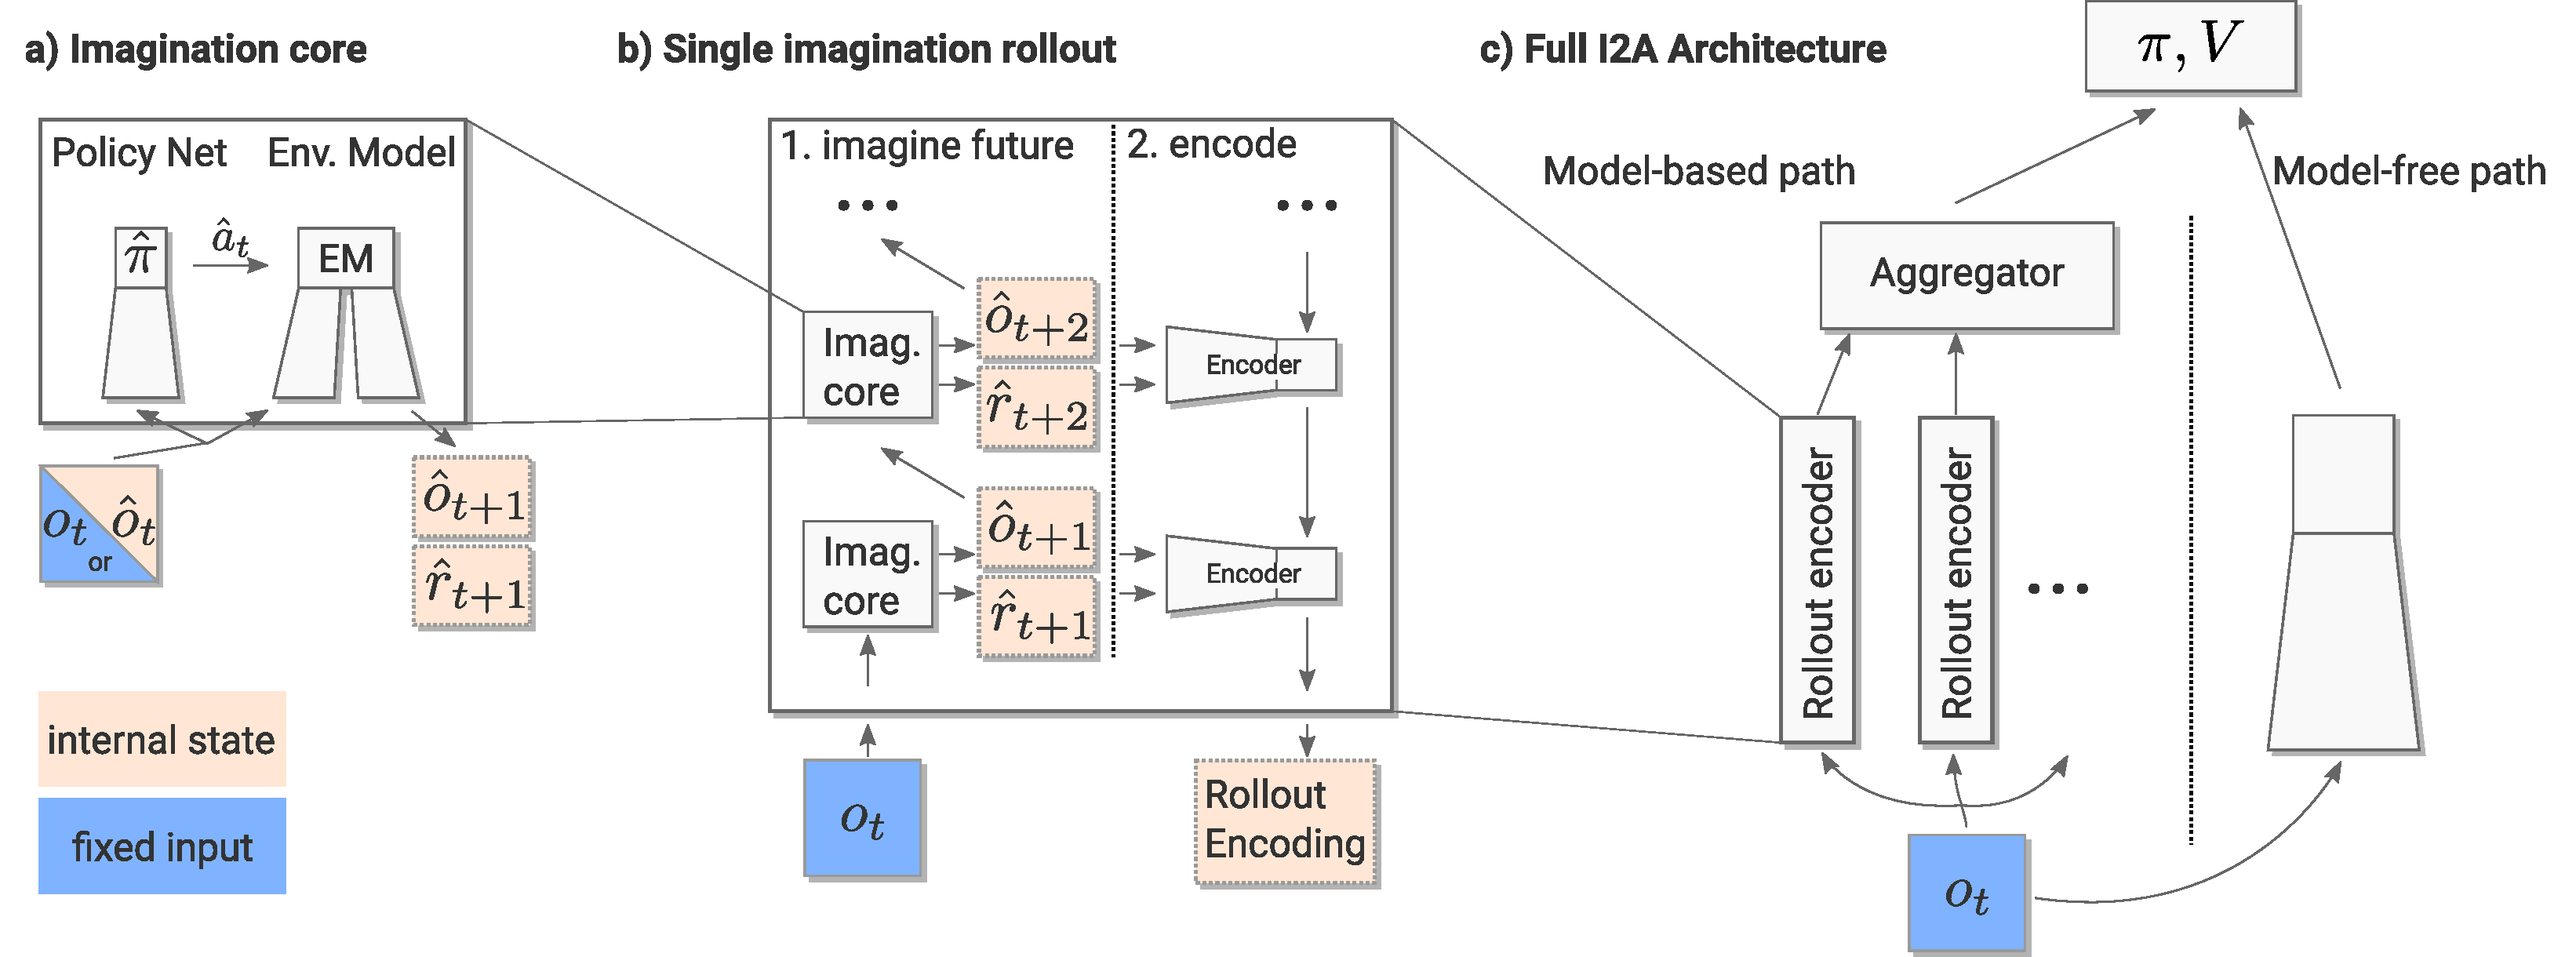
\includegraphics[scale=0.3]{i2a}
\caption{I2A architecture}
\end{figure*}

\section{Dataset}
We use the Arcade Learning Environment (ALE) to simulate playing Atari games. ALE has been integrated
into OpenAI Gym, which provides a standardized interface for taking actions and retrieving the resulting new
state, reward, etc. The game's state is simply the RGB image of a frame at a given point in time.

Before image data is fed into any part of the network, it is normalized in a way that is more convenient for training.
In particular, the top the image is removed, since it is only used to display the players' scores, pixels of which are
unlikely to be useful features. In addition, the top and bottom border color is changed from white to black, since
it is the same color as the ball. The idea is to help the network distinguish between the two types of pixels.
See Figure \ref{screenshots} below.

\begin{figure}[h]
\centering
\begin{subfigure}[b]{.2\textwidth}
  \centering
  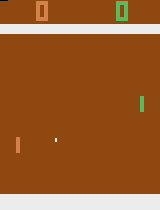
\includegraphics[scale=0.5]{unnormalized}
  \caption{Original image}
  \label{fig:unnormalized}
\end{subfigure} 
\begin{subfigure}[b]{.2\textwidth}
  \centering
  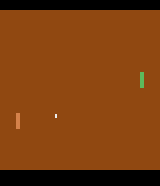
\includegraphics[scale=0.5]{normalized}
  \caption{After normalization}
  \label{fig:normalized}
\end{subfigure} \hfill
\caption{Pong screenshots before and after normalization}
\label{screenshots}
\end{figure}

The OpenAI Gym API provides rewards and states, so we work with this data when training our model.
Actions are taken with the \verb|step| function, which returns the resulting data.

\section{Methodology}

The model is trained in three phases. First, a model-free agent is trained using 

\subsection{Model-free agent}

\subsection{Environment model}

\subsection{I2A}

\section{Results}

\section{Discussion}

\end{document}